% Basic info about your document: a4 paper, 11pt font size, article style.
\documentclass[a4paper, 11pt]{article}

\usepackage{graphicx} % Enables adding figures
\usepackage[a4paper, margin=18mm]{geometry} % Let's you adjust the margins
\usepackage[T1]{fontenc} % Font helvetica
\usepackage[scaled]{helvet}
\usepackage{authblk} % multiauthor
\usepackage{multirow} % table
\usepackage[table,xcdraw]{xcolor}
\usepackage{float} % position des figures,table
\usepackage[backend=biber,style=numeric,sorting=none]{biblatex} % bibliographie
\usepackage{fancyhdr} % footer
\usepackage{caption} % caption
\usepackage{multicol} % multicolonne
\usepackage{adjustbox}
\usepackage{pdfpages}

%Setup bibliographie
\addbibresource{bibliographie.bib} % utilise bibliographie.bib pour la bibliographie

%Setup figure
\graphicspath{ {./figure/} } % relative path for figure

\renewcommand\familydefault{\sfdefault} % set font for all document
\captionsetup[table]{name=Tableau} % Rename table
\renewcommand*\contentsname{Table des matières} % Rename table of contents
\setlength\parindent{0pt} % remove indent in new line

%Setup Titre, auteur et date
\title{
    \vspace{-2.5cm}
    \centering\includegraphics[scale=0.5]{Logos\_Hepia.png}\\
    \centering\rule{17cm}{0.1mm}\vspace*{0.4in}\\
    \centering Projet thématique MOON}
\renewcommand\Authands{ et } % replace "and" by "et" in author
\author[1]{AYRINHAC Elisa}
\author[2]{DROUIN Clément}
\author[3]{JOUCLARD Charly}
\affil[1]{HEPIA, MT2, elisa.ayrinhac@hes-so.ch}
\affil[2]{HEPIA, MT2, clement.drouin@hes-so.ch}
\affil[3]{HEPIA, MT2, charly.jouclard@hes-so.ch}
\date{28 avril 2023}

%Setup header, footer
\pagestyle{fancy}
\fancyhead{} % clear all header fields
\renewcommand{\headrulewidth}{0pt} % no line in header area
\fancyfoot{} % clear all footer fields
\renewcommand{\footrulewidth}{1pt}
\newcommand{\changefont}{\fontsize{9}{11}\selectfont}
\newcommand{\TheAuthor}{AYRINHAC Elisa, DROUIN Clément, JOUCLARD Charly}
\fancyfoot[C]{\changefont\TheAuthor}
\fancyfoot[R]{\changefont\thepage}
\fancyfoot[L]{\changefont Projet thématique MOON}

\begin{document}

%Entete
\maketitle
\thispagestyle{empty}
\begin{center}
    \rule{\textwidth}{0.1mm}
\end{center}
%Introduction
\vspace{-1cm}
\section*{Introduction}
Ce rapport detail le projet thématique de deuxième année de bachelor
microtechnique de HEPIA option Bio-ingénierie.
Cette année notre cliente, Mme Loussert-Fonta Céline est une biologiste travaillante
sur l'endométriose, une maladie encore
peu connue mais très commune, touchant environ 1 femme sur 10.\\
Cette pathologie se caractérise par le développement du tissu semblable
à l'endomètre hors de l'utérus.
Ces tissus peuvent proliférer dans les organes voisins comme les ovaires;
l'intestin, la vessie ou même les poumons.
Les symptômes varient énormément entre les femmes mais ont retenu, le
plus souvent, celui de la douleur
extrême provoqué par la croissance de ces tissus.\\
Les objectifs du projet sont, d'une part, de mettre en application les
connaissances acquises durant nos études, mais également de développer de
nouvelles compétences comme la gestion de projet.
D'autre part, ce projet contribue à développer la recherche sur
l'endométriose et servira de support pour le \\
"project MOON : endoMetriosis Organoids to vOice up woman paiN".\\
Le but de notre projet est de créer un bio-chip qui permettrait d'étudier
les tissus de l'endomètre in vitro durant un cycle utérin. Cela signifie, imaginer, concevoir, fabriquer,
et tester un dispositif capable se recrée
les conditions d'un utérus (Température, humidité, concentration d'hormones, etc...)
\vspace{1cm}
\maketitle
\thispagestyle{empty}
\begin{center}
    \rule{\textwidth}{0.1mm}
\end{center}
\newpage
%Table des matieres
\tableofcontents
\newpage
%Debut rapport
\section{Etudes préliminaire}
\subsection{Biologie}
\subsubsection{Contexte}
Pour que l'expérience soit optimale, le client a besoin de suivre l'évolution d'un tissu d'endomètre sur la
durée d'un cycle endométrial.
Le système doit être compact et permettre l'observation des cellules en culture ainsi que la possibilité de
collecter des cellules et du milieu de culture pour analyse.
Afin mieux comprendre comment concevoir un appareil correspondant à la demande du client, une courte
introduction biologique est nécessaire.
\subsubsection{L'endomètre}
\begin{figure}[H]
    \centering
    \resizebox{0.5\linewidth}{!}{\includegraphics{Schema\_endomètre.jpg}}
    \caption{Localisation de l'endomètre dans l'utérus}
    \label{fig:Schema_endomètre}
\end{figure}
L'endomètre est un épithélium qui compose une partie de l'appareil reproducteur féminin, il tapisse les
parois de la cavité utérine et est composé de 3 couches :
\begin{itemize}
    \item Le myomètre qui est la fondation de l'endomètre.
    \item la couche basale qui contient les glandes et les tissu conjonctifs.
    \item la couche fonctionnelle.
\end{itemize}
Cette dernière couche est celle qui vois sa taille changer durant le cycle menstruel.
\subsubsection{Le cycle menstruel}
"Le cycle menstruel est l'ensemble des phénomènes physiologiques,
survenant le plus souvent de façon périodique, qui préparent l'organisme de la femme à une éventuelle
fécondation.
La connaissance du cycle menstruel est importante pour aborder l'étude des troubles de la menstruation,
dans l'exploration de l'infertilité et dans la mise en œuvre des techniques de procréation médicalement
assistées."
\cite{Cycle_menstruel}\\
L'hypothèse émise par la biologiste serait qu'il y a corrélation en le cycle hormonal et l'apparition
de kystes dus à l'endométriose.
Durant le cycle utérin, le taux d'hormonal de la femme varie selon les jours. Cela permet
au corps de réguler la période de croissance de l'endomètre, puis de déclencher l'ovation et enfin
S'il n'y a pas eu fécondation, de déclencher les menstruations.
\begin{figure}[H]
    \centering
    \resizebox{0.5\linewidth}{!}{\includegraphics{cycle\_menstruel.png}}
    \caption{Graphique montrant le cycle menstruel avec ces variation hormonal et ce que
        cela implique}
    \label{fig:Cycle menstruel}
\end{figure}
Comme vu dans la figure 2, les 4 hormones présentent dans le cycle sont :
\begin{itemize}
    \item La progestérone.
    \item Les estrogéne, notamment l'estradiol.
    \item La LH pour luteinizing hormone.
    \item La FSH pour follicle stimulating hormone.
\end{itemize}
La consigne est de reproduire les cycles de concentration de l'estradiol et de la progestérone.
Car ce sont les hormones suspectées dans l'apparition de l'endométriose. Cela signifie
recrée les conditions d'homéostasie des cellules ainsi que les conditions de
concentration de ce cycle et les appliquer à des cellules in vitro.
Afin de répondre au mieux à cette problématique un état de l'art de la culture
cellulaire sera établie ainsi qu'un inventaire des techniques présentent au campus biotech qui
pourraient être utile dans notre projet.
\newpage
\subsection{Etat de l'art}

\subsubsection{Incubateur}
Actuellement la culture cellulaire est un procédé connu et maitriser par l'Homme qui consiste à placer des cellules dans
un milieu de culture afin de les faire proliférer.
Cette méthode permet d'avoir des colonies de cellule pouvant aller jusqu'à former des organoïdes pouvant être utilisés
à des fins de recherche. Les organoïdes se comportant de manière similaire à l'organe miniaturisé.
Peu importe l'objectif, la méthode de culture garde toujours un objectif d'homéostasie et un objectif de prolifération. Dans la pratique cela revient
à placer dans un incubateur une colonie de cellules contenue dans un milieu nutritif.
Pour maintenir de bonnes conditions on place ces échantillons dans l'enceinte d'un incubateur qui permet d'isoler les cellules du milieu extérieur tout
en maintenant les constantes de températures, d'humidité et de CO2 de façon optimale.
Les incubateurs professionnels sont des machines de précision, asservis qui permettent de régler précisément toutes les conditions de leurs enceintes;
cela permet de chercher l'expression de certains phénotypes au sein des colonies.
Ils sont aussi dotés de sécurités notamment en matière de ventilation afin de protéger les cellules et le biologiste. Toutefois cette précision rend le matériel cher.
Il faut compter entre 5 000 CHF et 15 000 CHF pour un incubateur professionnel.
L'incubateur fait maison sont moins précise mais permette une personnalisation complète en matière de condition de culture.
Toutefois même si cela reste compliqué à construire dans sa totalité, il est assez simple de stabiliser la température et l'humidité.
Ces machines permettant de créer une atmosphère apte à la reproduction cellulaire toutefois il nous faut quelque chose qui contient les cellules et leur milieu nutritif.
il faut des instruments de culture biocompatible.
\subsubsection{Matériau biocompatible}
On appelle matériau biocompatible, les matériaux qui ont la capacité à ne pas interférer;
ne pas dégrader, le milieu biologique dans lequel ils sont utilisés. Dans notre cas, il faut
que le lieu d'accueil des cellules ne dégrade en rien leurs fonctionnements.
Actuellement les zones de culture sont
\begin{itemize}
    \item Les boites de pétris.
    \item Les écouvillons.
    \item La verrerie de chimie.
    \item Dans les labo d'HEPIA à la FCBG des biochip en PMMA, un polymere biocompatible.
\end{itemize}
Cette liste n'est pas exaustive, tout comptenant fait d'un matériau biocompatible peut en théorie
accueillir des cellules.
\subsubsection{Fluidique}
La fluidique est une partie importante dans la survie des cellules, c'est grace à elle que les
nutriments sont acheminés jusqu'à la zone de culture.
Elle se compose de tous les éléments comprenant du fluide, tel que :
\begin{itemize}
    \item Les réservoirs.
    \item Les pompes.
    \item les tuyaux.
    \item les vannes.
\end{itemize}
Les tuyaux utilisés à la FCBG sont de qualités médicales, c'est-à-dire qui sont biocompatibles. Ils ne diffusent pas
dans le milieu de culture, et ils ne sont pas sensibles aux méthodes de stérilisation.
\newpage
\subsection{Aperçu du projet}
\subsubsection{Besoins}
On peut voir avec la figure \ref{fig:bete_corne} que le système conçu va permettre au biologiste d'étudier l'influence des hormones sur du tissu endométrial.
\begin{figure}[H]
    \centering
    \resizebox{\linewidth}{!}{\includegraphics{bete\_corne.png}}
    \caption{Bête à corne}
    \label{fig:bete_corne}
\end{figure}
\subsubsection{Fonctions}
\begin{table}[H]
    \centering
    \begin{tabular}{|
            >{\columncolor[HTML]{CBCEFB}}l |l|}
        \hline
        \multicolumn{1}{|c|}{\cellcolor[HTML]{CBCEFB}\textbf{N°}} & \textbf{Fonction}                                 \\ \hline
        FP1                                                       & Maintenir les cellules en vie                     \\ \hline
        FP2                                                       & Intégrer des concentrations spécifiques d'hormone \\ \hline
        FC3                                                       & Observer les cellules au microscope               \\ \hline
        FC4                                                       & Alimenter le système en énergie                   \\ \hline
        FC5                                                       & Réaliser un système autonome                      \\ \hline
        FC6                                                       & Résister au milieu imposer par les cellules       \\ \hline
        FC7                                                       & Utiliser un matériau biocompatible                \\ \hline
        FC8                                                       & Respecter le budget                               \\ \hline
        FC9                                                       & Assurer un cycle de 28 jours                      \\ \hline
    \end{tabular}
    \caption{Fonctions à assurer}
\end{table}
\begin{figure}[H]
    \centering
    \resizebox{\linewidth}{!}{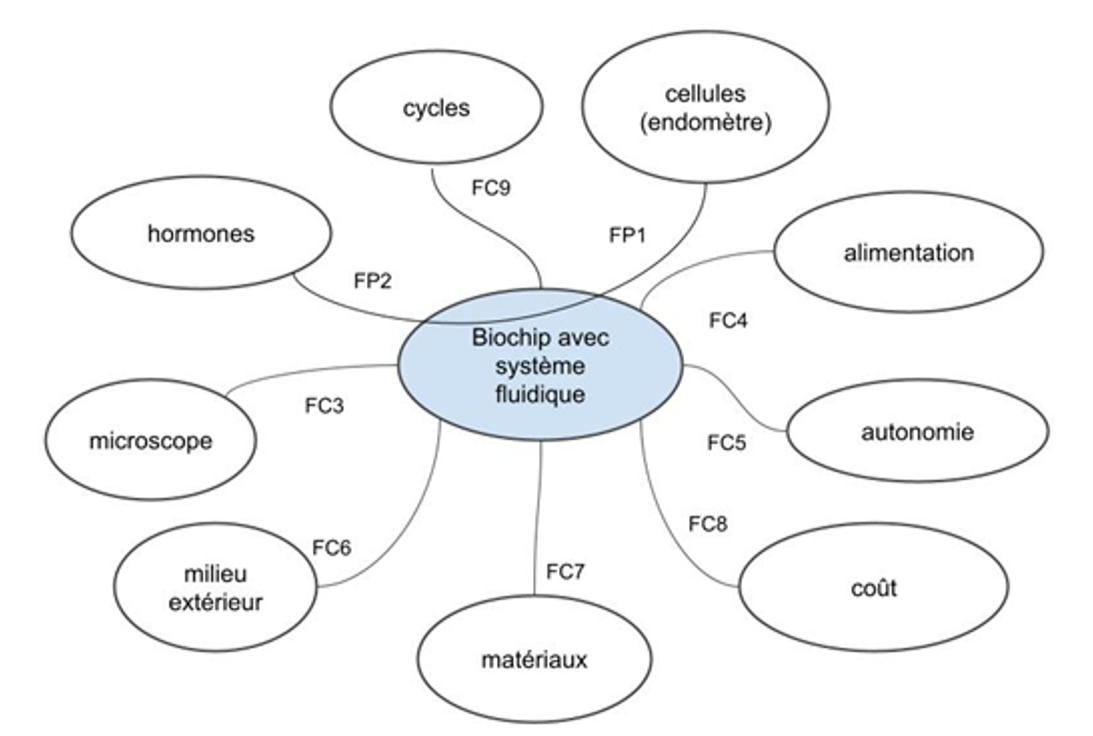
\includegraphics{pieuvre.png}}
    \caption{Diagramme pieuvre avec les fonctions associés}
    \label{fig:pieuvre}
\end{figure}
\subsection{Cahier des charges}
La première fonction à prendre en compte est la survie des cellules.
Pour cela, notre système devra respecter les paramètres suivants :
\begin{itemize}
    \item une température de 37°C
    \item un pH de 7
    \item un renouvellement du milieu de culture de 1 ml par jours
    \item atténué toute variation de milieu
    \item la Biocompatibilité du milieu
\end{itemize}
Pour ce qui est du système fluidique, il permet l'apport du milieu de culture à la cellule et donc nécessite de répondre aux points suivants :
\begin{itemize}
    \item un système étanche
    \item un écoulement laminaire
    \item un système de purge
    \item un système d'injection d'hormones
    \item un mélangeur pour éviter des pics de concentration
    \item une pompe pour un système dynamique
\end{itemize}
Enfin, le système dans sa globalité devra assurer :
\begin{itemize}
    \item une autonomie de 28 jours minimum
    \item une zone transparente permettant l'observation des cellules
\end{itemize}
\subsection{Catalogue de solutions}
\subsubsection{Gestion des nutriments, déchets et de la concentration des hormones}
\begin{table}[H]
    \centering
    \begin{tabular}{|l|l|l|}
        \hline
        \multicolumn{1}{|c|}{\textbf{Solution}}        & \textbf{Avantages}                                                                                                     & \textbf{Inconvénients}                                                                                                             \\ \hline
        Seringues auto-poussés                         & \begin{tabular}[c]{@{}l@{}}-Précis\\ -Facile d'utilisation\\ -Facilement programmable\\ -Réponse linéaire\end{tabular} & \begin{tabular}[c]{@{}l@{}}-Energie\\ -Limité en quantité\\ -Espace\end{tabular}                                                   \\ \hline
        \rowcolor[HTML]{CBCEFB}
        Pompe péristaltiques\cite{pompe_peristaltique} & -Déjà présent au labo                                                                                                  & \begin{tabular}[c]{@{}l@{}}-Peu précis\\ -Energie\end{tabular}                                                                     \\ \hline
        Système de goutte à goutte                     & \begin{tabular}[c]{@{}l@{}}-Low-cost\\ -Economique en énergie\end{tabular}                                             & \begin{tabular}[c]{@{}l@{}}-Précision\\ -A pression atmosphérique\\ -Complexité d'asservissement\\ -Réponse chaotique\end{tabular} \\ \hline
    \end{tabular}
    \caption{Solutions pour la gestions des nutriments, déchets et des hormones}
\end{table}
\subsubsection{Contrôler l'environnement extérieur}
\begin{table}[H]
    \centering
    \begin{tabular}{|l|l|l|}
        \hline
        \multicolumn{1}{|c|}{\textbf{Solution}} & \textbf{Avantages}                                                                                        & \textbf{Inconvénients}                                                                      \\ \hline
        \rowcolor[HTML]{CBCEFB}
        Incubateur                              & \begin{tabular}[c]{@{}l@{}}-Constante externe stable\\ -A disposition\\ -Retour d'expérience\end{tabular} & \begin{tabular}[c]{@{}l@{}}-Placé dans l'incubateur\\ -Protéger l'électronique\end{tabular} \\ \hline
        Système autonome                        & -Pas de dépendance                                                                                        & \begin{tabular}[c]{@{}l@{}}-Compliqué à réaliser\\ -Energivore\\ -Coût\end{tabular}         \\ \hline
    \end{tabular}
    \caption{Solutions pour gérer l'environnement extérieur}
\end{table}
\subsubsection{Cultiver les cellules}
\begin{table}[H]
    \centering
    \begin{tabular}{|l|l|l|}
        \hline
        \multicolumn{1}{|c|}{\textbf{Solution}} & \textbf{Avantages}                                                                                         & \textbf{Inconvénients}                                                             \\ \hline
        \rowcolor[HTML]{CBCEFB}
        Bio-chip en PMMA                        & \begin{tabular}[c]{@{}l@{}}-Usinage\\ -Retour d'expérience\\ -Sur mesure\\ -Fluidique intégré\end{tabular} & \begin{tabular}[c]{@{}l@{}}-Assemblage par couche\\ -Long à fabriquer\end{tabular} \\ \hline
        Boîte de pétris                         & \begin{tabular}[c]{@{}l@{}}-Coût\\ -Stérilité\end{tabular}                                                 & -Pas de circulation de fluide                                                      \\ \hline
    \end{tabular}
    \caption{Solutions pour le milieu de culture}
\end{table}
\subsubsection{Circulation du fluide}
\begin{table}[H]
    \centering
    \begin{tabular}{|l|l|l|}
        \hline
        \multicolumn{1}{|c|}{\textbf{Solution}} & \textbf{Avantages}                                                                                            & \textbf{Inconvénients}                                           \\ \hline
        \rowcolor[HTML]{CBCEFB}
        Pompe péristaltique                     & \begin{tabular}[c]{@{}l@{}}-Déjà présent au labo\\ -Facile d'utilisation\\ -Pas de contamination\end{tabular} & \begin{tabular}[c]{@{}l@{}}-Débit limité\\ -Energie\end{tabular} \\ \hline
        Gravité                                 & \begin{tabular}[c]{@{}l@{}}-Pas besoin de matériel spécifique\\ -Pas besoin d'alimentation\end{tabular}       & -Compliqué à mettre en oeuvre                                    \\ \hline
    \end{tabular}
    \caption{Solutions pour injecter les différents fluides}
\end{table}
\subsubsection{Mélanger les fluides}
\begin{table}[H]
    \centering
    \begin{tabular}{|l|l|l|}
        \hline
        \multicolumn{1}{|c|}{\textbf{Solution}} & \textbf{Avantages}                                                                                                           & \textbf{Inconvénients}                                                                                  \\ \hline
        \rowcolor[HTML]{CBCEFB}
        Mélangeur hydrostatique "2D"            & \begin{tabular}[c]{@{}l@{}}-Economique\\ -Facilité d'intégration\\ -Compact\\ -Volume sur mesure\\ -Modélisable\end{tabular} & \begin{tabular}[c]{@{}l@{}}-A créer\\ -Perte de charge\end{tabular}                                     \\ \hline
        Mélangeur hydrostatique "3D"            & \begin{tabular}[c]{@{}l@{}}-Economique\\ -Facilité d'intégration\\ -Compact\\ -Volume sur mesure\\ -Modélisable\end{tabular} & \begin{tabular}[c]{@{}l@{}}-A créer\\ -Perte de charge\\ -Usinage\end{tabular}                          \\ \hline
        Mélangeur magnétique                    & \begin{tabular}[c]{@{}l@{}}-Déjà présent au labo\\ -Facilement nettoyable\\ -Gestion de la puissance\end{tabular}            & \begin{tabular}[c]{@{}l@{}}-Espace\\ -Biocompatibilité\\ -Non modélisable\\ -Non pilotable\end{tabular} \\ \hline
    \end{tabular}
    \caption{Solutions pour assurer l'homogénéité des liquides}
\end{table}
\subsubsection{Analyser les concentrations}
\begin{table}[H]
    \centering
    \begin{tabular}{|l|l|l|}
        \hline
        \multicolumn{1}{|c|}{\textbf{Solution}} & \textbf{Avantages}                                                                                                                  & \textbf{Inconvénients}                                                                           \\ \hline
        \rowcolor[HTML]{CBCEFB}
        Colorimètre externe                     & \begin{tabular}[c]{@{}l@{}}-Facilité d'intégration\\ -Précis\\ -Déjà présent au labo\end{tabular}                                   & \begin{tabular}[c]{@{}l@{}}-Aucune donnée interne\\ -Nécessite présence utilisateur\end{tabular} \\ \hline
        Colorimètre interne                     & \begin{tabular}[c]{@{}l@{}}-Retour en temps réel\\ -Gain de précision de l'asservissement\\ -Donnée interne au système\end{tabular} & \begin{tabular}[c]{@{}l@{}}-A créer\\ -Précision\end{tabular}                                    \\ \hline
    \end{tabular}
    \caption{Solutions pour contrôler les concentrations}
\end{table}
\subsubsection{Contrôler le système (microcontrôleur)}
\begin{table}[H]
    \centering
    \begin{tabular}{|l|l|l|}
        \hline
        \multicolumn{1}{|c|}{\textbf{Solution}} & \textbf{Avantages}                                                                                                                                      & \textbf{Inconvénients}                                                                                                                           \\ \hline
        Arduino Uno                             & \begin{tabular}[c]{@{}l@{}}-Facilité d'utilisation\\ -Flexible\end{tabular}                                                                             & \begin{tabular}[c]{@{}l@{}}-Pas de stockage interne\\ -Pas de contrôle à distance\\ -Pas de possibilité d'utiliser python\\ -14 pin\end{tabular} \\ \hline
        \rowcolor[HTML]{CBCEFB}
        Raspberry Pi                            & \begin{tabular}[c]{@{}l@{}}-Retour en temps réel\\ -Contrôlable à distance\\ -Stockage interne\\ -Utilisation possible de Python\\ -40 pin\end{tabular} & -Faible disponibilité                                                                                                                            \\ \hline
    \end{tabular}
    \caption{Solutions pour commander le système}
\end{table}
\subsubsection{Alimentation}
\begin{table}[H]
    \centering
    \begin{tabular}{|l|l|l|}
        \hline
        \multicolumn{1}{|c|}{\textbf{Solution}} & \textbf{Avantages} & \textbf{Inconvénients}                                              \\ \hline
        \rowcolor[HTML]{CBCEFB}
        Secteur                                 & -Disponibilité     & -Toujours branché                                                   \\ \hline
        Batteries                               & -Portable          & \begin{tabular}[c]{@{}l@{}}-Prix\\ -Recharge compliqué\end{tabular} \\ \hline
    \end{tabular}
    \caption{Solutions pour alimenter le bio-chip}
\end{table}
\subsection{Schéma bloc du système}
\begin{figure}[H]
    \centering
    \resizebox{\linewidth}{!}{\includegraphics{schema\_block.png}}
    \caption{Schéma bloc du système}
    \label{fig:schema_block}
\end{figure}
\subsection{Déroulé du projet}
insert diagramme de gant
\subsection{Choix pour le projet}
Afin de réaliser la culture de cellules de l'endomètre, tout en respectant le cahier
des charges, la conception d'un bio-chip sur-mesure devient une . Pour ce faire on va utiliser différents
outils disponibles dans le laboratoire afin de diminuer les coûts. Certaines pièces devront être
fabriqués afin de répondre au besoin comme le boitier du bio-chip.
Pour accueillir les cellules un boitier en PMMA sera conçu et usiner sur
place grâce à la découpe laser qui se trouve dans le campus.
Pour la régulation de l'environnement l'utilisation d'un incubateur présent dans le laboratoire sera
utilisés pour accueillir les cellules afin de diminuer le cout de fabrication.
Pour la partie commandée, l'utilisation d'un micro-ordinateur type Raspberry pie permettra de contrôler
Les constantes du bio-chip. Pouvant contrôler celui-ci à distance et étant plus puissance, le raspberry a
De multiples avantages face à l'ardu ino UNO.
Pour un apport d'hormones et de nutriment précis les pousses seringues qui sont disponibles
dans le laboratoire, vont être incorporer au système, toutefois l'éventualité d'utiliser des pompes à là
place n'est pas écartée.
Les pompes fournies par HEPIA, pour le projet, permettrons de créer un flux au sein du biochip.
L'ensemble du bio-chip sera alimenté par le secteur afin de limiter les coûts de fabrication et éviter
de devoir développer un système avec une batterie.

\newpage
\section{Conception mécanique}
\subsection{Mélangeur hydrostatique}
\subsubsection{Simulation fluidique}
Dans cette partie porté sur la simulation et de la modélisation d'un mélangeur statique
permettant de rendre le mélange homogène avant de l'envoyer sur les cellules.
Afin de déterminer la forme du mélangeur une courte recherche a été faite sur la simulation fluide de créo.
Dans l'industrie, les mélangeurs statiques sont des composants de fluidique en 3 dimensions conçue pour
perturber l'écoulement et ainsi créé des turbulences.
Cela a pour but de mélanger le fluide sans utiliser de composant actif tel qu'une pompe, un moteur;
ou un mélangeur magnétique.
\begin{figure}[H]
    \centering
    \resizebox{0.4\linewidth}{!}{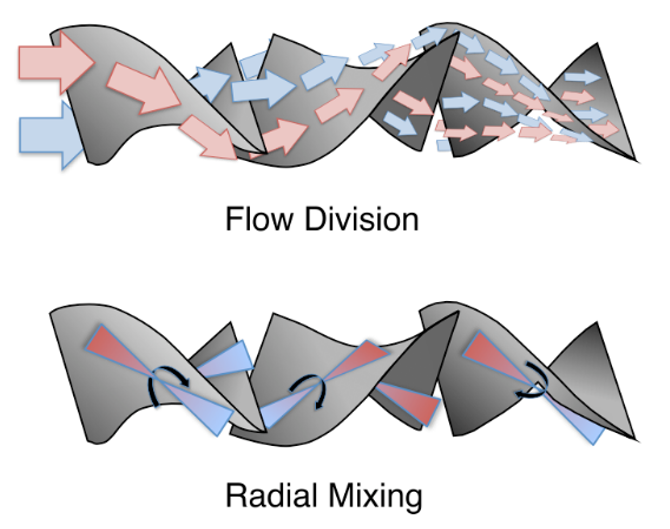
\includegraphics{simulation1.png}}
    \caption{Schéma montrant comment ce mélange un fluide}
    \label{fig:simulation1}
\end{figure}
Une première étape de conception fut donc d'essayer de comprendre à quoi pourrait bien ressembler ce
type de mélangeur en 2D.
On sait de par la mécanique des fluides que la pression et la vitesse d'écoulement sont liée à la
géométrie du milieu d'écoulement. Ainsi pour mélanger les fluides il faut "perturber" le flux afin de faire
varier la vitesse de manière hétérogène.
Ainsi différents mélangeurs ont été modélisés afin d'observer le comportement du fluide alors
d'une simulation.
De plus le mode de fabrication le plus simple étant la découpe LASER il a fallu adapter la forme
de ceux-ci afin qu'il soit réalisable en entier à la découpeuse LASER du campus.
\newline
\begin{multicols}{2}
    \begin{figure}[H]
        \centering
        \resizebox{0.95\linewidth}{!}{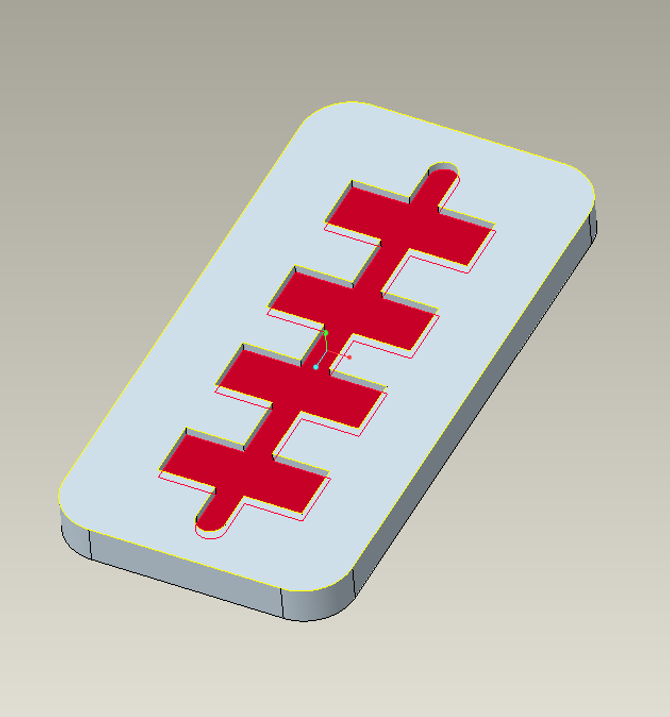
\includegraphics{CAO_prototype_melangeur.png}}
        \caption{CAO du mélangeur avec chicanes}
        \label{fig:CAO_prototype_melangeur}
    \end{figure}
    \begin{figure}[H]
        La figure \ref{fig:CAO_prototype_melangeur} montre la première étape de recherche;
        le premier mélangeur était juste composé d'un chemin direct auquel ont été ajoutées
        des cavités latérales.
        Le flux de liquide assimilé à de l'eau dans la simulation entre par en dessous et sort par au-dessus;
        et les conditions de pression sont celles données dans la datasheet de la pompe, étant donné
        que le mélangeur sera placé juste derrière la pompe.
    \end{figure}
\end{multicols}
\newpage
\begin{multicols}{2}
    \begin{figure}[H]
        \centering
        \resizebox{0.95\linewidth}{!}{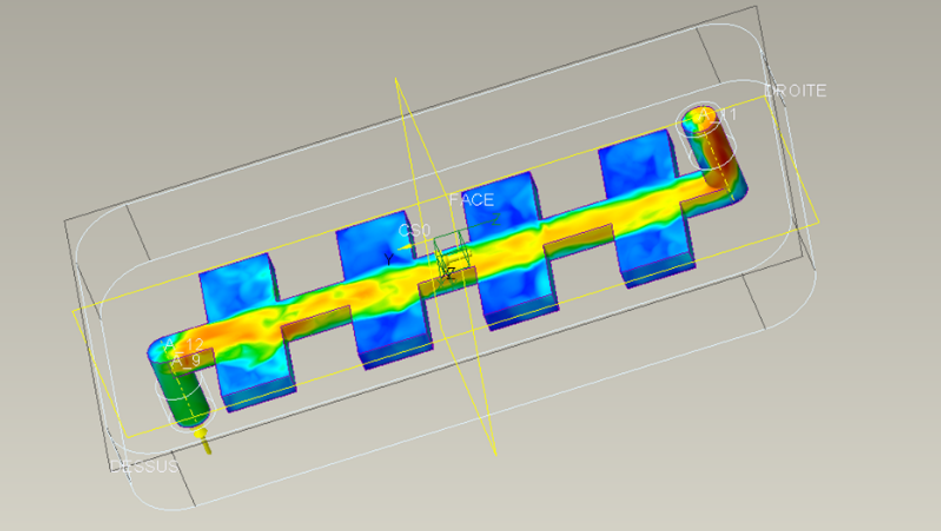
\includegraphics{simulation2.png}}
        \caption{Première simulation fluidique}
        \label{fig:simulation2}
    \end{figure}
    \begin{figure}[H]
        La figure \ref{fig:simulation2} montres un résultat de simulation.
        Les couleurs représentent la vitesse du flux de liquide, ici la simulation avait juste pour but de
        tester les fonctionnalités de créo. Toutefois il y a des zones (en bleu) ou le liquide est statique
        et des zones (Orange) ou le liquide ses deplace plus rapidement.
        L'idée a ensuite été de séparer le flux en deux et de les recombiner pour créer des turbulences.
        Une autre version avait pour idée de détendre et de comprimer le flux afin de créer des
        turbulences.
    \end{figure}
\end{multicols}

\begin{figure}[H]
    \centering
    \resizebox{0.5\linewidth}{!}{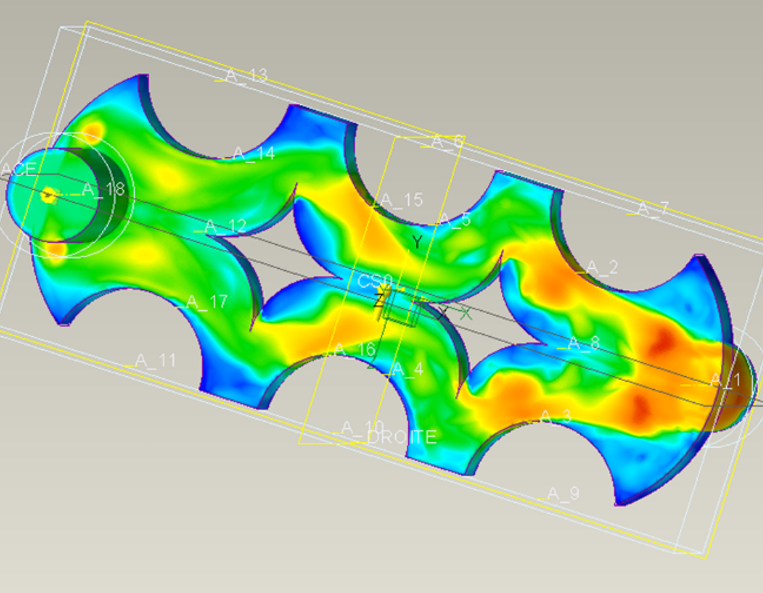
\includegraphics{simulation5.png}}
    \caption{Simulation fluidique avec chicanes et obstacles}
    \label{fig:simulation5}
\end{figure}
La figure \ref{fig:simulation5} montre l'importance de placer un obstacle au centre du flux, de plus la variation
de section vient ajouter des perturbations. C'est ce schéma qui est retenu pour la forme du mélangeur.
Les variations de section vont être accentuées et le bloc central sera en un seul morceau afin de facilité les
découpes.
Le principe de montage repose sur celui deja utilisé dans les laboratoires de HEPIA. Le melangeur sera composé de 3
couches;
\begin{itemize}
    \item Une première couche servant de socle, dotée de trous dans lesquels des goupilles pourront etres insérées.
    \item Une couche centrale contenant la forme du mélangeur, c'est-à-dire les bords et le centre.
    \item Une dernière couche permettant de refermer le mélangeur et de fixer les raccords de fluidique.
\end{itemize}
\newpage

\subsubsection{CAO du mélangeur}
Apres plusieurs simulations, les choix se sont tourné vers un mélangeur comportant l'entrée et la sortie de chaque
coté du mélangeur. Le flux est séparer en deux par la partie centrale, puis les flux sont accélérés séparément parréduction
de la section découlement. Des zones plus vaste, (contenant plus de liquide) sont laiser colontairement afin de profoqué un diférence de vitesse
entre le liquide présent dans ces zones et celui qui arrive. Enfin le chemin fluide n'est composée que de partie de courbe,
cela permet de limiter l'apparition de bulles.
\begin{multicols}{2}
    \begin{figure}[H]
        \centering
        \resizebox{\linewidth}{!}{\includegraphics{CAO\_melangeur\_couche2.png}}
        \caption{Couche central du mélangeur}
        \label{fig:CAO_melangeur_couche2}
    \end{figure}
    \begin{figure}[H]
        \centering
        \resizebox{\linewidth}{!}{\includegraphics{CAO\_melangeur.png}}
        \caption{Mélangeur hydrostatique}
        \label{fig:CAO_melangeur}
    \end{figure}
\end{multicols}
Notre conception est basée sur un principe de sandwich, une première épaisseur permettant l'étanchéité, le support et le guidage des autres couches.
Une couche centrale munit d'un détrompeur composer d'un élément externe guider par deux goupilles extérieures, et un élément interne guidé par les goupilles intérieures.
Et enfin une dernière couche permettant de fermer le tout, toujours guider par les deux goupilles externes.
L'adhésion et l'étanchéité sera assuré par une couche adhésive déposer sur les plaques.
\subsection{Zone de culture}
\begin{figure}[H]
    \centering
    \resizebox{0.5\linewidth}{!}{\includegraphics{CAO\_cellule.png}}
    \caption{bio-chip pour les cellules}
    \label{fig:CAO_cellule}
\end{figure}
Pour le biochip contenant les cellules visibles sur la figure \ref{fig:CAO_cellule}, nous avons choisi d'utiliser l'assemblage en plusieurs couches de PMMA.
Celui-ci contient 4 couches d'épaisseur différentes pour répondre à certaines contraintes.
Nous utiliserons des goupilles, pour être sûr que les différents éléments soient bien alignés.

\newpage
\begin{multicols}{2}
    \begin{figure}[H]
        \centering
        \resizebox{\linewidth}{!}{\includegraphics{CAO\_cellule\_couche1.png}}
        \caption{CAO de la première couche}
        \label{fig:CAO_cellule_couche1}
    \end{figure}
    \begin{figure}[H]
        \centering
        \resizebox{\linewidth}{!}{\includegraphics{CAO\_cellule\_couche2.png}}
        \caption{CAO de la seconde couche}
        \label{fig:CAO_cellule_couche2}
    \end{figure}
\end{multicols}
La couche du dessous fait 0.3 mm d'épaisseur pour facilité l'observation des cellules au microscope.
La 2e couche est prévu pour contenir les cellules mais sera supprimer car elle crée des angles droits qui risque d'endommager les cellules.
\begin{multicols}{2}
    \begin{figure}[H]
        \centering
        \resizebox{\linewidth}{!}{\includegraphics{CAO\_cellule\_couche3.png}}
        \caption{CAO de la troisième couche}
        \label{fig:CAO_cellule_couche3}
    \end{figure}
    \begin{figure}[H]
        \centering
        \resizebox{\linewidth}{!}{\includegraphics{CAO\_cellule\_couche4.png}}
        \caption{CAO de la quatrième couche}
        \label{fig:CAO_cellule_couche4}
    \end{figure}
\end{multicols}
La 3e couche permet au fluide contenant les hormones et nutriment de circuler la où seront accroché les cellules.
L'entrée du fluide est plus étroite que la sortie pour éviter des problèmes de surpression.
Et enfin la dernière couche contient les trous pour chasser les connecteur Luer lock, permettant de relier le bio chip contenant les cellules au reste du système par l'intermédiaire de tuyaux.
Les angles devront être arrondit pour éviter d'endommager les cellules.
\subsection{Support des réservoirs}
Désormais le rendu physique projet devient très claire,
celui-ci sera composer d'un boitier auxquelles sera fixé les trois pompe,
les quatre tube comprenant les hormones, le liquide de culture neuf, et usagé.
Ce boitier sera lui aussi découper au LASER et au besoin renforcé par des pièces
imprimé en 3D.
Il ne contiendra pas l'électronique, celui-ci sera placer en dehors de l'incubateur
et relier au système via un câble.
Il est à noter qu'il manque les électrovannes, qui ont été modéliser et qui seront
placer de l'autre côté des pompes.
\begin{multicols}{2}
    \begin{figure}[H]
        \centering
        \resizebox{\linewidth}{!}{\includegraphics{CAO\_reservoir1.png}}
        \caption{CAO du porte réservoir version 1}
        \label{fig:CAO_reservoir1}
    \end{figure}
    \begin{figure}[H]
        \centering
        \resizebox{\linewidth}{!}{\includegraphics{CAO\_reservoir2.png}}
        \caption{CAO du porte réservoir version 2}
        \label{fig:CAO_reservoir2}
    \end{figure}
\end{multicols}
\begin{figure}[H]
    \centering
    \resizebox{0.4\linewidth}{!}{\includegraphics{CAO\_electrovanne.png}}
    \caption{CAO des électrovannes}
    \label{fig:CAO_electrovanne}
\end{figure}
\subsubsection{Le boitier découpable au LASER}
Le boitier à été concus pour etre entièrment découper au LASER. Pour cela chaque face du boitier à été modélisé de facon à se qu'elle s'emboite entre elles une fois assemblé.
Pour des questions de maintient, 8 petites équerres de maintient à visser ont été concus
et les plaques serons collées entre elles par de la colle à plexiglass.
On peut aussi imaginer ne pas fixer une des plaque mais la vissée et placer un joint papier.
Cela permettrais d'avoir la possibilité d'ouvrir le boitier sans le casser.
\begin{figure}[H]
    \centering
    \resizebox{\linewidth}{!}{\includegraphics{CAO\_boitier\_decoupe\_LASER.png}}
    \caption{CAO du boitier à découper au LASER}
    \label{fig:CAO_boitier_decoupe_LASER}
\end{figure}
De plus, deux support à imprimer en 3D,ont été ajoutées pour fixer le melangeur et
la zone de culture.
Ces support permettrons de fixer la zone de culuture et de pouvoir la retirer pour
faire des observation.

\newpage
\subsection{Assemblage des biochips}
Pour réaliser l’assemblage du mélangeur et du biochip qui contiendra les cellules,
la première étapes a été de découper chaque éléments dans des plaques de PMMA.
Afin de facilité l’assemblage, seul la couche du milieu est recouverte de colle
sur ces deux faces. La deuxième étape consiste à assembler le tout.
Les goupilles du gabarit (voir figure \ref{fig:gabarit}) permettent l’alignement
des 3 différentes couches. Une fois les 3 couches superposer,
il faut s’assurer que celle-ci sont correctement collé entre elles.
Pour cela, les trois couches sont pressé entre elles à l’aide d’un rouleau.
Enfin, les luer-lock sont emboiter dans le boichip avec de la colle époxy.
\begin{multicols}{3}
    \begin{figure}[H]
        \centering
        \resizebox{\linewidth}{!}{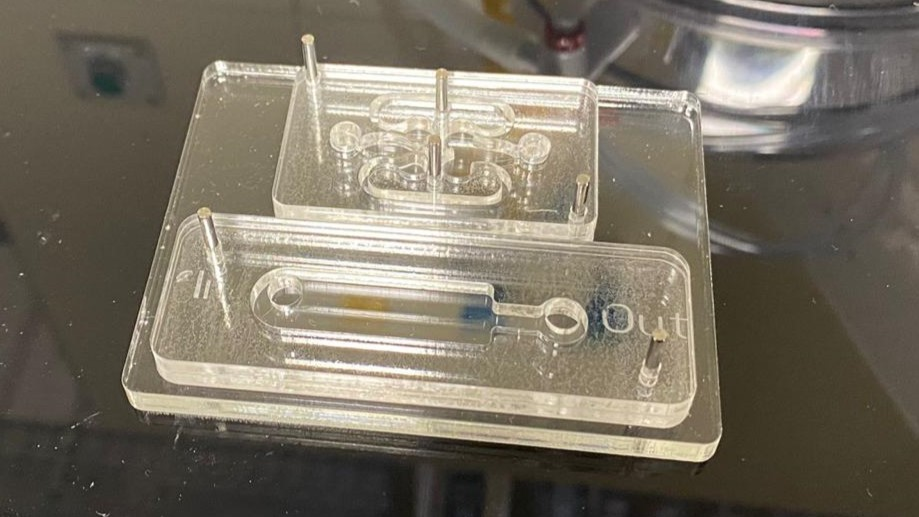
\includegraphics{gabarit.JPG}}
        \caption{Photo du gabarit et des biochips}
        \label{fig:gabarit}
    \end{figure}
    \begin{figure}[H]
        \centering
        \resizebox{\linewidth}{!}{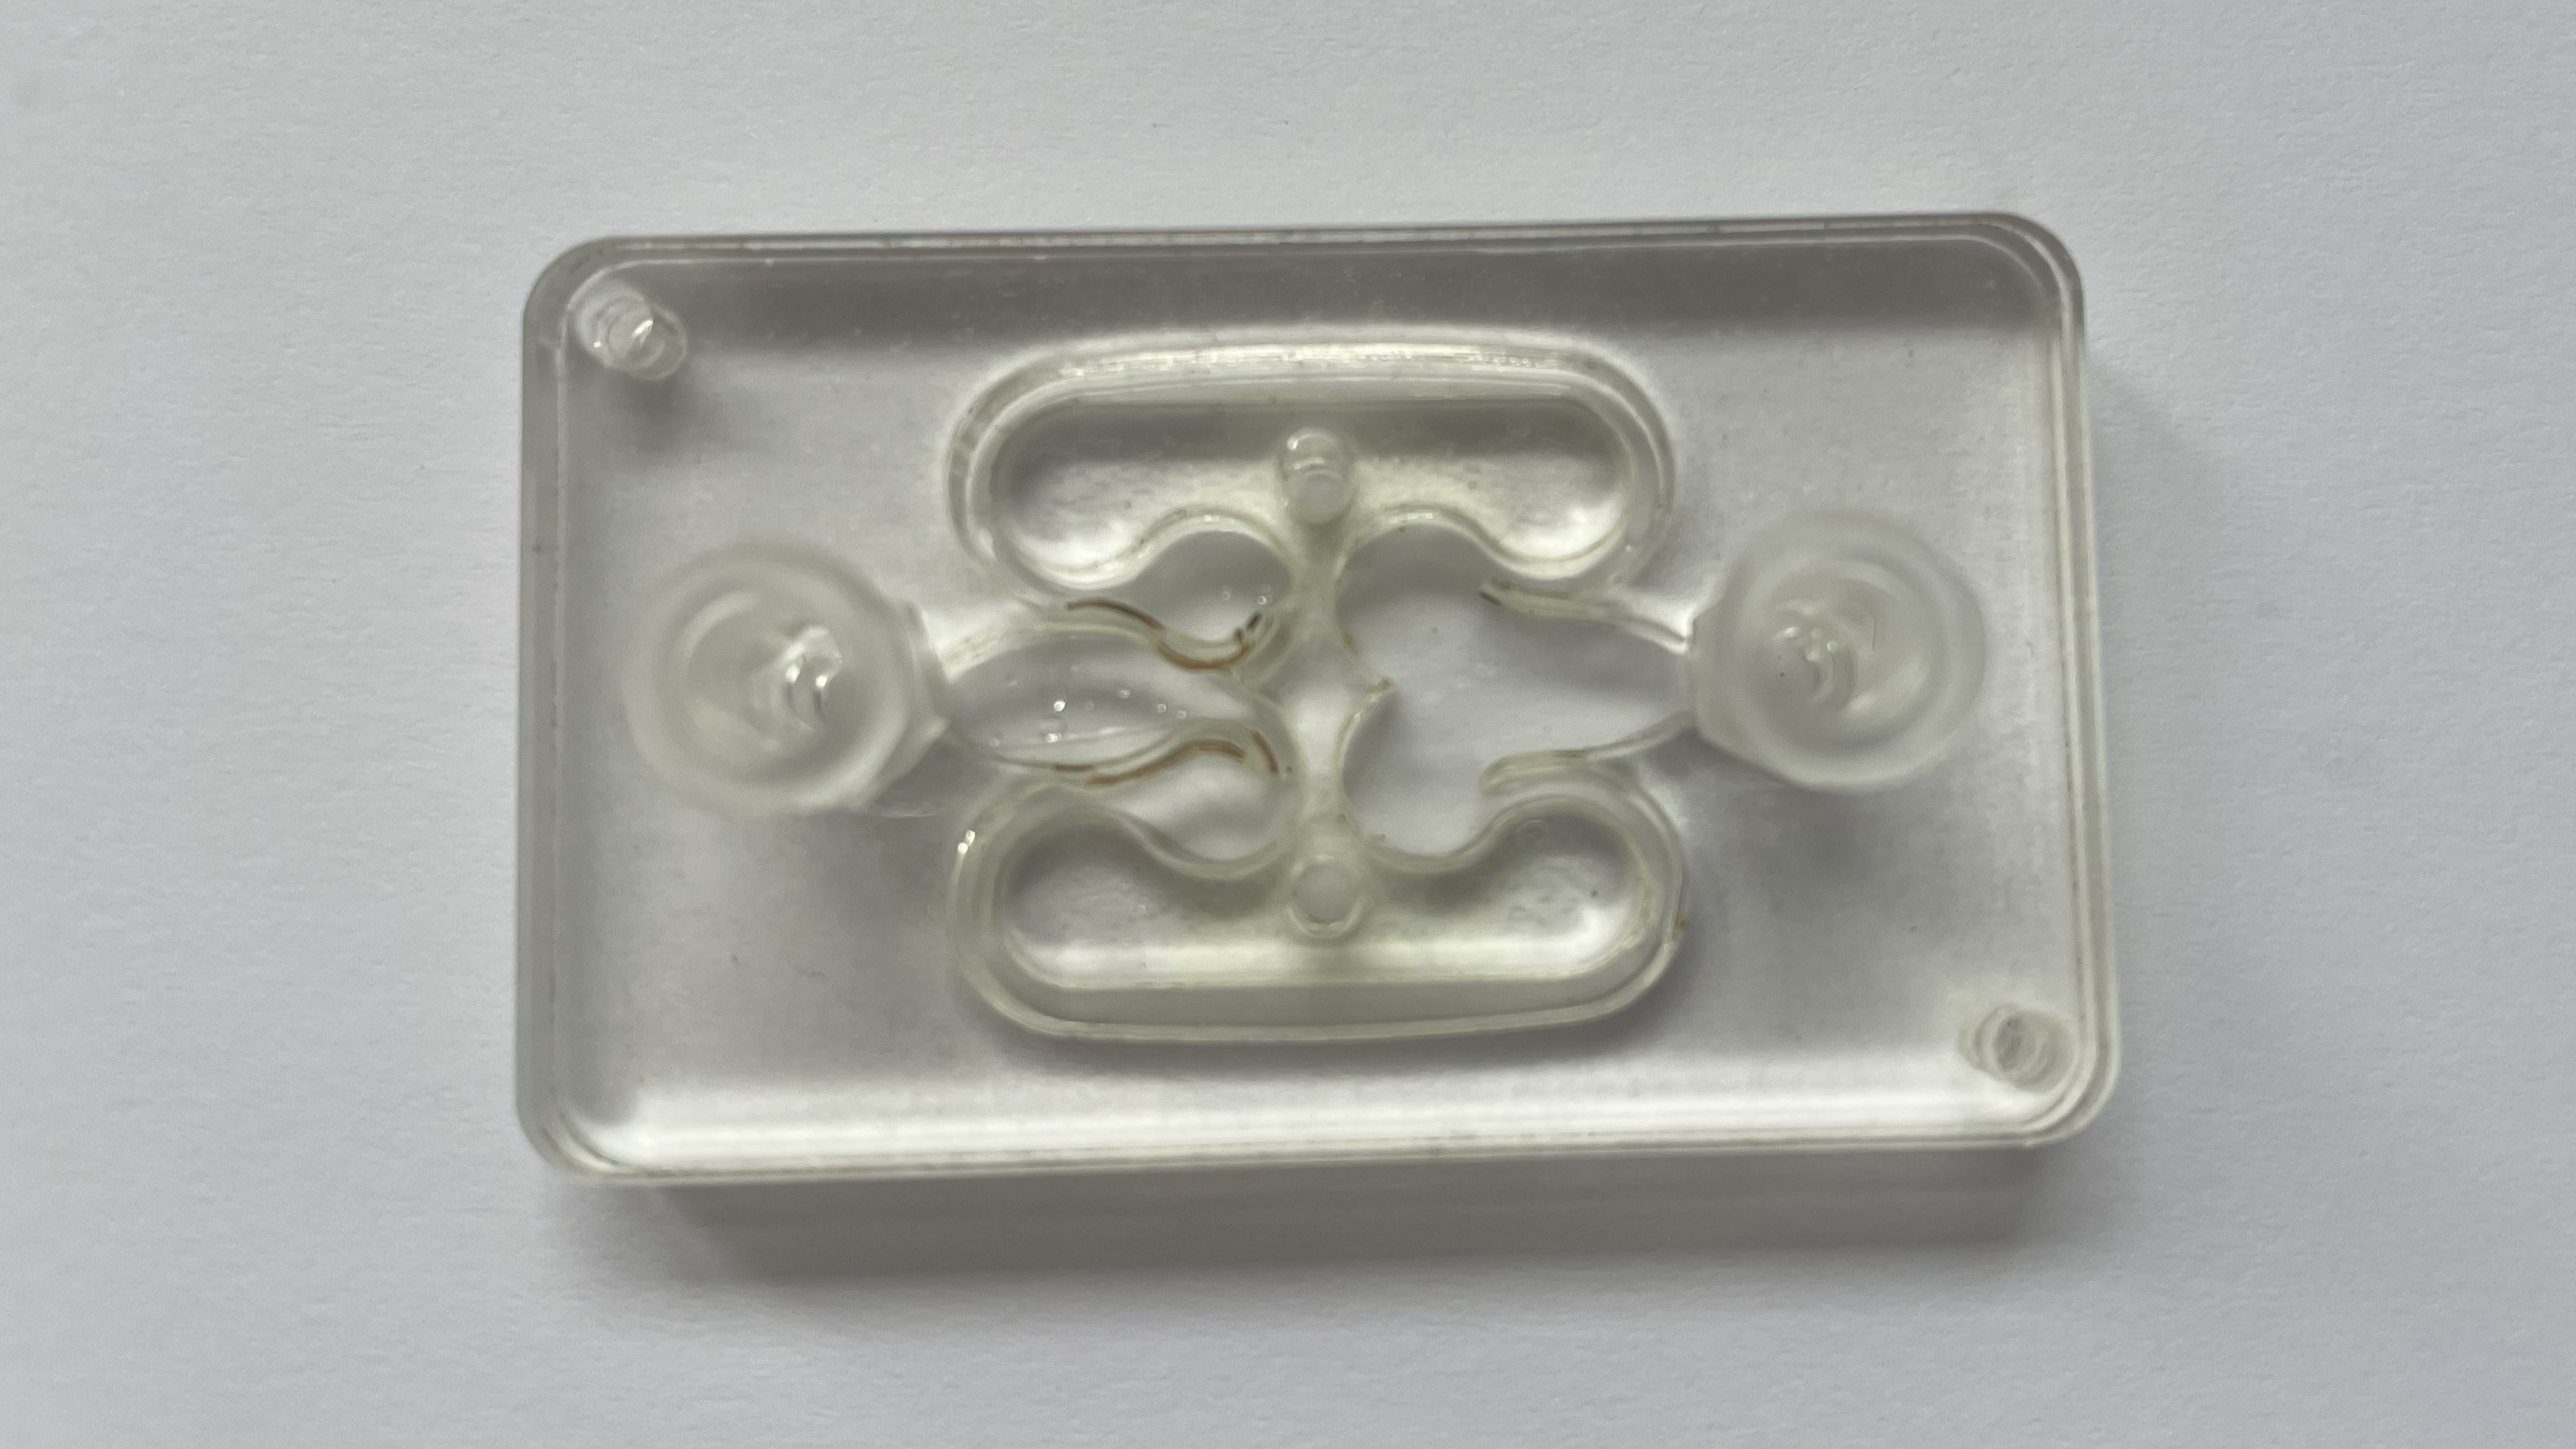
\includegraphics{melangeur.jpg}}
        \caption{Photo de l'assembage du mélangeur}
        \label{fig:melangeur}
    \end{figure}
    \begin{figure}[H]
        \centering
        \resizebox{\linewidth}{!}{\includegraphics{biochip\_cellulesV1.jpg}}
        \caption{Photo de l'assembage du biochip cellules}
        \label{fig:cellules}
    \end{figure}
\end{multicols}
\subsubsection{Le biochip cellules}
\begin{multicols}{2}
    \begin{figure}[H]
        \centering
        \resizebox{\linewidth}{!}{\includegraphics{fluide\_cellulesV1.jpg}}
        \caption{Photo du test fluidique}
        \label{fig: fluide_cellules}
    \end{figure}
    \begin{figure}[H]
        \centering
        \resizebox{\linewidth}{!}{\includegraphics{reste\_fluide\_cellulesV1.jpg}}
        \caption{Photo des restes de liquide}
        \label{fig:reste_cellules}
    \end{figure}
\end{multicols}
Après avoir injecté du fluide dans le biochip, celui-ci ne fuit pas.
Cependant, le test a montré une mauvaise optimisation de l'espace.
En effet, comme le montre la photo de la figure 4, le liquide reste
bloqué à certains endroits. Pour optimiser la circulation du fluide,
une nouvelle version de ce biochip a été modélisée.
\newpage
\subsubsection{Modelisation biochip cellules version 2}
\begin{multicols}{2}
    \begin{figure}[H]
        \centering
        \resizebox{\linewidth}{!}{\includegraphics{CAO\_cellulesV2.png}}
        \caption{CAO assemblage biochip cellules V2}
        \label{fig: CAO_cellulesV2}
    \end{figure}
    \begin{figure}[H]
        \centering
        \resizebox{\linewidth}{!}{\includegraphics{CAO\_cellules\_milieu\_V2.png}}
        \caption{CAO milieu du biochip cellules V2}
        \label{fig:milieu_cellulesV2}
    \end{figure}
\end{multicols}
Les entrées et sorties du fluide ont le même diamètre que les trous pour insérer les embouts luer-lock, afin d'éviter d'avoir une zone inutile autour de ces embouts.
De plus, pour la zone plus large qui accueillera les cellules, les angles à 90° ont été remplacés par des angles à 45°. Cela devrait éviter la formation de bulles d'air.
\subsubsection{Le mélangeur}
Les premiers tests du mélangeur ont été effectués en faisant circuler du liquide à l'intérieur, à l'aide de seringues.
\begin{figure}[H]
    \centering
    \resizebox{\linewidth}{!}{\includegraphics{fuite\_melangeur.PNG}}
    \caption{Photo test fluidique mélangeur}
    \label{fig:fuite_melangeurV1}
\end{figure}
Comme on peut observer sur la \label{fig:fuite_melangeur} le liquide s'infiltre dans l'intercouche ce qui cause une fuite
par un trou de fabrication.
\subsubsection{CAO mélangeur version 2}
Le premier mélangeur fuyait, cela était probablement dû à une surpression qui causait
l'infiltration du liquide dans l'intercouche. Ainsi dans l'optique de pouvoir commencer
Le test le plus rapidement possible, un nouveau mélangeur, plus simple, a été modéliser.
Celui-ci a pour but d'être plus solide, d'être encore usinable au LASER, et d'utiliser un volume moindre.
\begin{multicols}{2}
    \begin{figure}[H]
        \centering
        \resizebox{\linewidth}{!}{\includegraphics{CAO\_melangeur\_V2\_couche1.png}}
        \caption{Premiere couche du melangeur V2}
        \label{fig: CAO_melangeur_V2_couche1}
    \end{figure}
    \begin{figure}[H]
        \centering
        \resizebox{\linewidth}{!}{\includegraphics{CAO\_melangeur\_V2\_couche2.png}}
        \caption{Deuxième couche du mélangeur V2}
        \label{fig:CAO_melangeur_V2_couche2}
    \end{figure}
\end{multicols}
L'idée de séparer puis de refusionner le flux est rester
sauf que le chemin est bien plus simple et les bords sont toujours
arrondits. Une section reduite permet une accélation du flux.
Les dimensions on été agrandi afin d'avoir 1cm de chaque coté ce
qui est deux fois plus que l'ancien.
\begin{multicols}{2}
    \begin{figure}[H]
        \centering
        \resizebox{\linewidth}{!}{\includegraphics{CAO\_melangeur\_V2\_couche3.png}}
        \caption{Dernière couche du melangeur V2}
        \label{fig: CAO_melangeur_V2_couche3}
    \end{figure}
    \begin{figure}[H]
        \centering
        \resizebox{\linewidth}{!}{\includegraphics{CAO\_melangeur\_V2.png}}
        \caption{L'assemblage du mélangeur V2}
        \label{fig:CAO_melangeur_V2}
    \end{figure}
\end{multicols}
Le nouveau mélangeur remplace l'ancien ainsi la piece
permettant la fixation du mélangeur au boitier à donc été ajusté.
\subsubsection{CAO boitier version 2}
\begin{figure}[H]
    \centering
    \resizebox{\linewidth}{!}{\includegraphics{CAO\_boitier\_decoupe\_LASER\_V2.png}}
    \caption{Boitier modifier pour accueillir le melangeur V2}
    \label{fig:CAO_boitier_V2}
\end{figure}
La figure \ref{fig:CAO_boitier_V2} montre le rendu final du prototype, il reste alors à le découper et à l'assembler.
\newpage
\section{Conception électronique et programmation}
\subsection{Carte d'alimentation version 1}
\begin{figure}[H]
    \centering
    \resizebox{\linewidth}{!}{\includegraphics{carte\_alimentation.png}}
    \caption{Montage électronique pour l'alimentation du Raspberry Pi et des pompes version 1}
    \label{fig:CAO_electronique_V1}
\end{figure}
L'alimentation de tous le biochip se fera via l'alimentation d'un Arduino de 60 W.
Il arrive sur la carte d'alimentation via la connectique circulaire JAlim.
U1 est un régulateur de tension à découpage de la marque TRACO, il permet de descendre la tension de 12V à 5V il sert à alimenter le Raspberry pi qui sera alimenter par ses pins GPIO.
Les moteurs seront contrôlés par les mosfet M1, M2 et M3.
Les moteurs seront branchés à la carte via des connecteurs circulaire afin que le système soit le plus flexible possible.
Les diodes D1, D2 et D3 sont des diodes de roues libres.
\newpage
\subsubsection{Carte d'alimentation version 2 et 3}
Lorsque nous avons testé la première version du circuit électronique nous avons remarqué que le montage ne fonctionnait pas.
En effet nous avons remarqué que le raspberry pi ne fournit pas assez de tension aux mosfets pour alimenter les pompes.
Pour pouvoir alimenter correctement les pompes une tension de 3,5 V est nécessaire à la "gate" des mosfets.
Cependant le raspberry pi ne peut fournir qu'une tension de 3,3 V via les pins qui sont contrôlables.
\begin{figure}[H]
    \centering
    \resizebox{\linewidth}{!}{\includegraphics{carte\_alimentationV2.png}}
    \caption{Montage électronique pour l'alimentation du Raspberry Pi et des pompes version 2}
    \label{fig:CAO_electronique_V2}
\end{figure}
Pour obtenir la tension adéquate nous avons amplifié le signal grâce à un AOP pour pouvoir piloter les pompes.
Les AOP devaient être alimentés via le 12 V du transformateur.
Après plusieurs essais infructueux nous avons remarqué que les AOP que nous avons choisies ne peuvent être alimentées par une alimentation non-symétrique.
En alimentant les amplificateurs via une alimentation de laboratoire stabilisé avec une tension symétrique +5/-5 V le montage fonctionnait correctement.
\begin{figure}[H]
    \centering
    \resizebox{\linewidth}{!}{\includegraphics{carte\_alimentationV3.png}}
    \caption{Montage électronique pour l'alimentation du Raspberry Pi et des pompes version 3}
    \label{fig:CAO_electronique_V3}
\end{figure}
Nous avons récupéré de nouveau amplificateurs qui sont compatibles en alimentation non-symétrique, pour éviter de devoir alimenter une partie du montage via une alimentation de laboratoire.
Comme nous avons reçu les nouveaux amplificateurs assez tardivement, nous n'avons pas eu le temps de tester le montage avec les nouveaux amplificateurs.
Si les amplificateurs ne conviennent pas nous resterons sur l'alimentation de laboratoire pour alimenter les amplificateurs.
\subsection{Programmation}
\subsubsection{GitHub}
On a mis en place un GitHub pour se partager les codes de programmation, le "repo" contient aussi une ébauche du guide d'utilisateur.
Le guide d'utilisateur contient actuellement uniquement les requirements pour le Raspberry pi ainsi que les commandes à utiliser.
\subsubsection{Raspberry Pi}
On a configuré le Raspberry pi 4 pour qu'on puisse se connecter dessus à distance à l'aide du protocole SSH.
On peut s'y connecter facilement dessus à partir du moment que l'on se trouve sur le même réseau wifi.
On peut lui transmettre des fichiers ainsi que récupérer des fichiers qui sont stockées dessus.
\subsubsection{Préparation des données}
Ce code permet de préparer les datas afin de pouvoir être utiliser par le logiciel qui contrôle le biochip.
Il a été conçu pour que l'utilisateur rentre un minimum de donner afin de gagner du temps.
Il permet de convertir un fichier csv que l'utilisateur aura créée au préalable avec les différents jalons de concentration en un fichier qui contient toutes les concentrations de l'expérience sur 28 jours.
Sur la figure \ref{fig:dataPreparation} on peut voir une représentation des données rentrées par l'utilisateur et les données produites par le programme.
\begin{figure}[H]
    \centering
    \resizebox{\linewidth}{!}{\includegraphics{representation\_data\_gen.png}}
    \caption{Données généré par le programme avec les données rentrées par l'utilisateur}
    \label{fig:dataPreparation}
\end{figure}
On peut l'utiliser directement sur un ordinateur puis envoyer le fichier généré sur le Raspberry pi ou bien on peut envoyer le fichier csv sur le Raspberry pi puis le généré directement sur le Raspberry pi.
Le fichier généré est un fichier de type ftr il n'est donc pas lisible directement ceci est fait afin de gagner en rapidité d'exécution et gagner du stockage.
Si on utilisait un fichier csv équivalent il contiendrait tellement de donnés qu'il faudrait plusieurs secondes pour le généré et il prendrait 10 fois plus de stockage.
Le fichier à préparer doit être présenter sous la forme :
\begin{table}[H]
    \centering
    \begin{tabular}{lll}
        Time & Conc1 & Conc2 \\
        0    & 1     & 1     \\
        2    & 6     & 8     \\
        10   & 2     & 1     \\
        15   & 4     & 2
    \end{tabular}
\end{table}
\subsubsection{Programme de test des moteurs}
Un code python permet de vérifier si le contrôle des moteurs fonctionne bien.
En plus de ça il permet d'effectuer les tests de débits des pompes.
Normalement il faudrait environ 30 minutes pour pouvoir tester les débits de toutes les pompes sur une plage de tension d'alimentation des pompes de 6 V à 12 V.
Le code qui permet de contrôler les pompes sera le même que celui dans le programme principal.
Cela va permettre de gagner du temps lors du développement de celui-ci.
\newpage
\section{Maquette final}
Cette dernière partie est une présentation du prototype final.
\subsection{Conception du chassis}
Le chassis utilisés ne sera pas celui présenter precedement car ce projet n'a besoins
d'une maquette fonctionnelle, il s'aggit un projet visant à démontrer que
le systeme fonctionne. La maquette n'ira pas dans l'incubateur, elle n'as pas
besoin d'être étanche.
Ainsi une CAO d'une maquette plus simple a été réaliser puis usiner.
\begin{multicols}{2}
    \begin{figure}[H]
        \centering
        \resizebox{0.95\linewidth}{!}{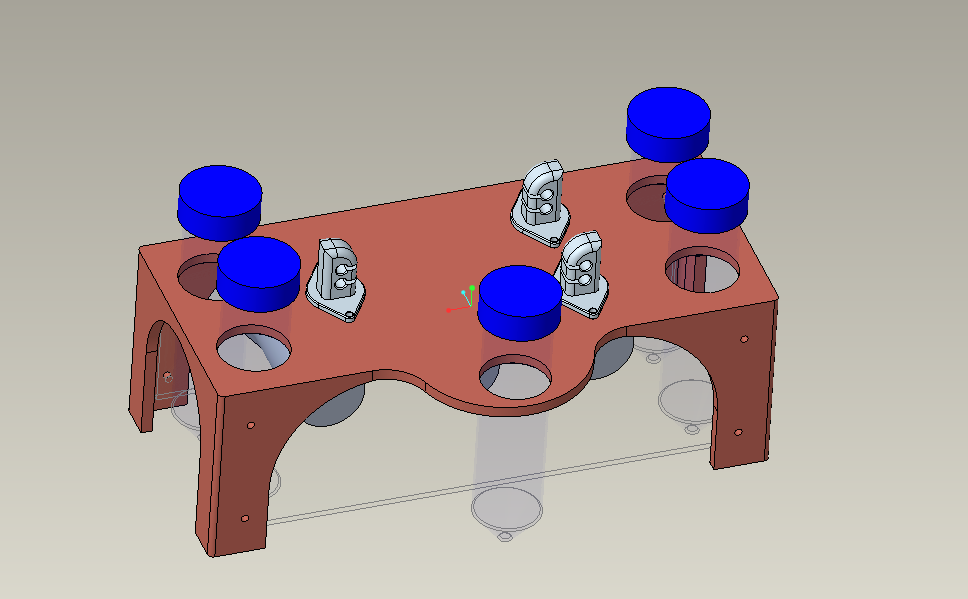
\includegraphics{CAO_final.png}}
        \caption{CAO final}
        \label{fig:CAO_final}
    \end{figure}
    \begin{figure}[H]
        \centering
        \resizebox{0.95\linewidth}{!}{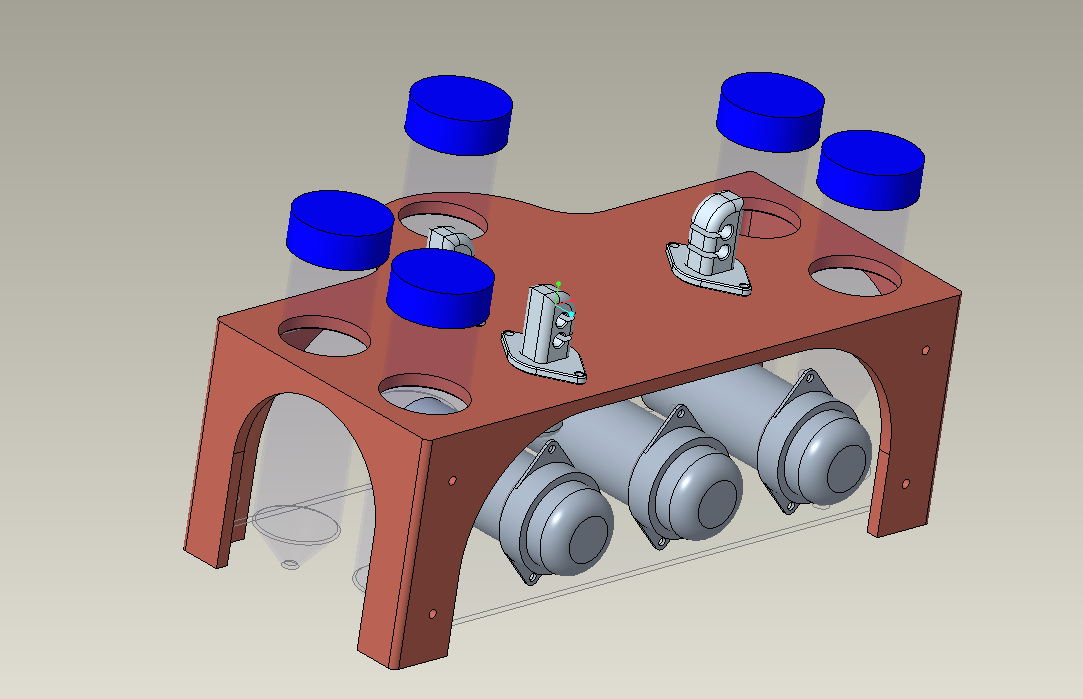
\includegraphics{CAO_final_dos.png}}
        \caption{CAO final vue des moteurs}
        \label{fig:CAO_final_dos}
    \end{figure}
\end{multicols}
Le châssis a été pensé pour être imprimable en 3D, la structure est renforcée avec deux
plaque de PMMA découper au LASER de 3 mm d'épaisseur. La structure est montée grace à
des vis M3 et des écrous. Une des Pâques latérales sera usinée afin d'accueillir les pompes.
Les électrovannes seront fixées sur la partie imprimée en 3D et fixées avec des vis M2.
Le plus grand changement réside dans l'abandon du mélangeur découper au LASER, en effet un 5éme réservoir a été ajouté pour servir de mélangeur. Celui-ci sera muni d'une entrée "compte-gouttes" qui
Consistera en un en bout monté sur le bouchon sans tube venant tomber dans le réservoir.
Pour la sortie il s'agira d'un tube allant au fond du mélangeur.
Le mélangeur fonctionnera comme une perfusion médicale, ce genre de dispositif est très efficace
mais possède une constante de temps de mélange relativement grande, celle-ci dépendant en
grande partie du volume engagé dans le système.
\begin{figure}[H]
    \centering
    \resizebox{0.95\linewidth}{!}{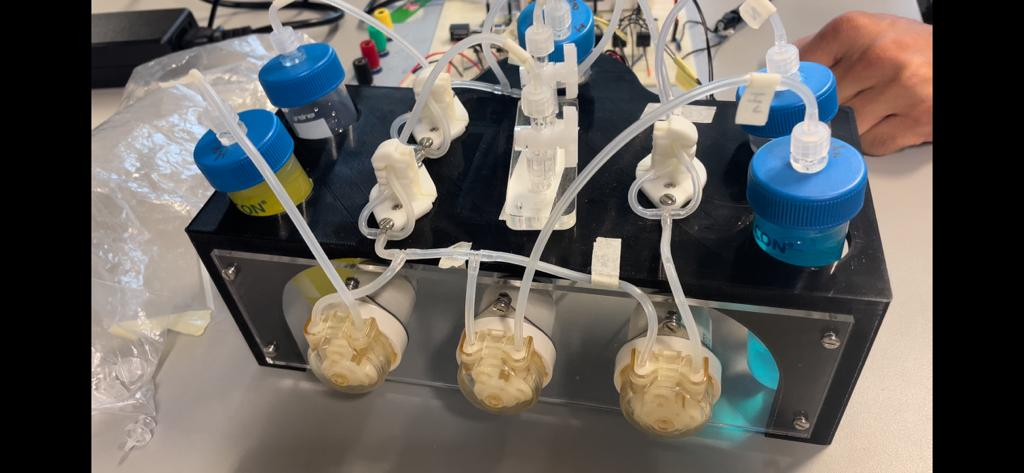
\includegraphics{Image_maquette_final.jpg}}
    \caption{Maquette final}
    \label{fig:Maquette}
\end{figure}
\newpage
\section{Conclusion}
La réalisation de ce projet a permis de mettre à profit nos connaissances afin de concevoir un système permettant de soumettre des cellules à un cycle de concentration d'hormones spécifique. Ce projet nous a enseigné les outils de gestion de projet, ce qui nous a conduit au développement du prototype final. Tout au long de ce projet en groupe, nous avons tiré des leçons de nos erreurs, améliorant ainsi notre efficacité.
\newline
Pour accueillir les cellules, nous avons conçu un biochip en PMMA, associé à un circuit fluidique. Ce circuit est composé de pompes et d'électrovannes, permettant de reproduire de manière contrôlée le cycle de concentration d'hormones.
\newline
L'ensemble du système est intégré dans un boîtier réalisé en impression 3D et en PMMA. Une version étanche de ce boîtier a été développée pour protéger les pompes et les électrovannes lorsqu'elle est placée dans l'incubateur, tandis que l'électronique de contrôle est placée en dehors de l'incubateur.
\newline
L'électronique est commandée par un Raspberry Pi 4. L'utilisateur peut interagir avec le système depuis son ordinateur grâce à la connexion WiFi. Il a ainsi la possibilité de transmettre un fichier CSV contenant des concentrations spécifiques, ce qui rend le système modulable et adaptable selon ses préférences.
\newline
Le prototype réalisé est fonctionnel, mais des améliorations peuvent être envisagées pour le rendre encore plus performant. Par exemple, la conception d'une carte PCB dédiée et d'un boîtier externe pour l'électronique contribuerait à améliorer la fiabilité et la robustesse du système.
\newline
En conclusion, ce système de fluidique offre une solution fonctionnelle pour soumettre des cellules à un cycle de concentration d'hormones spécifique. Des améliorations peuvent être envisagées pour améliorer les performances.

\newpage

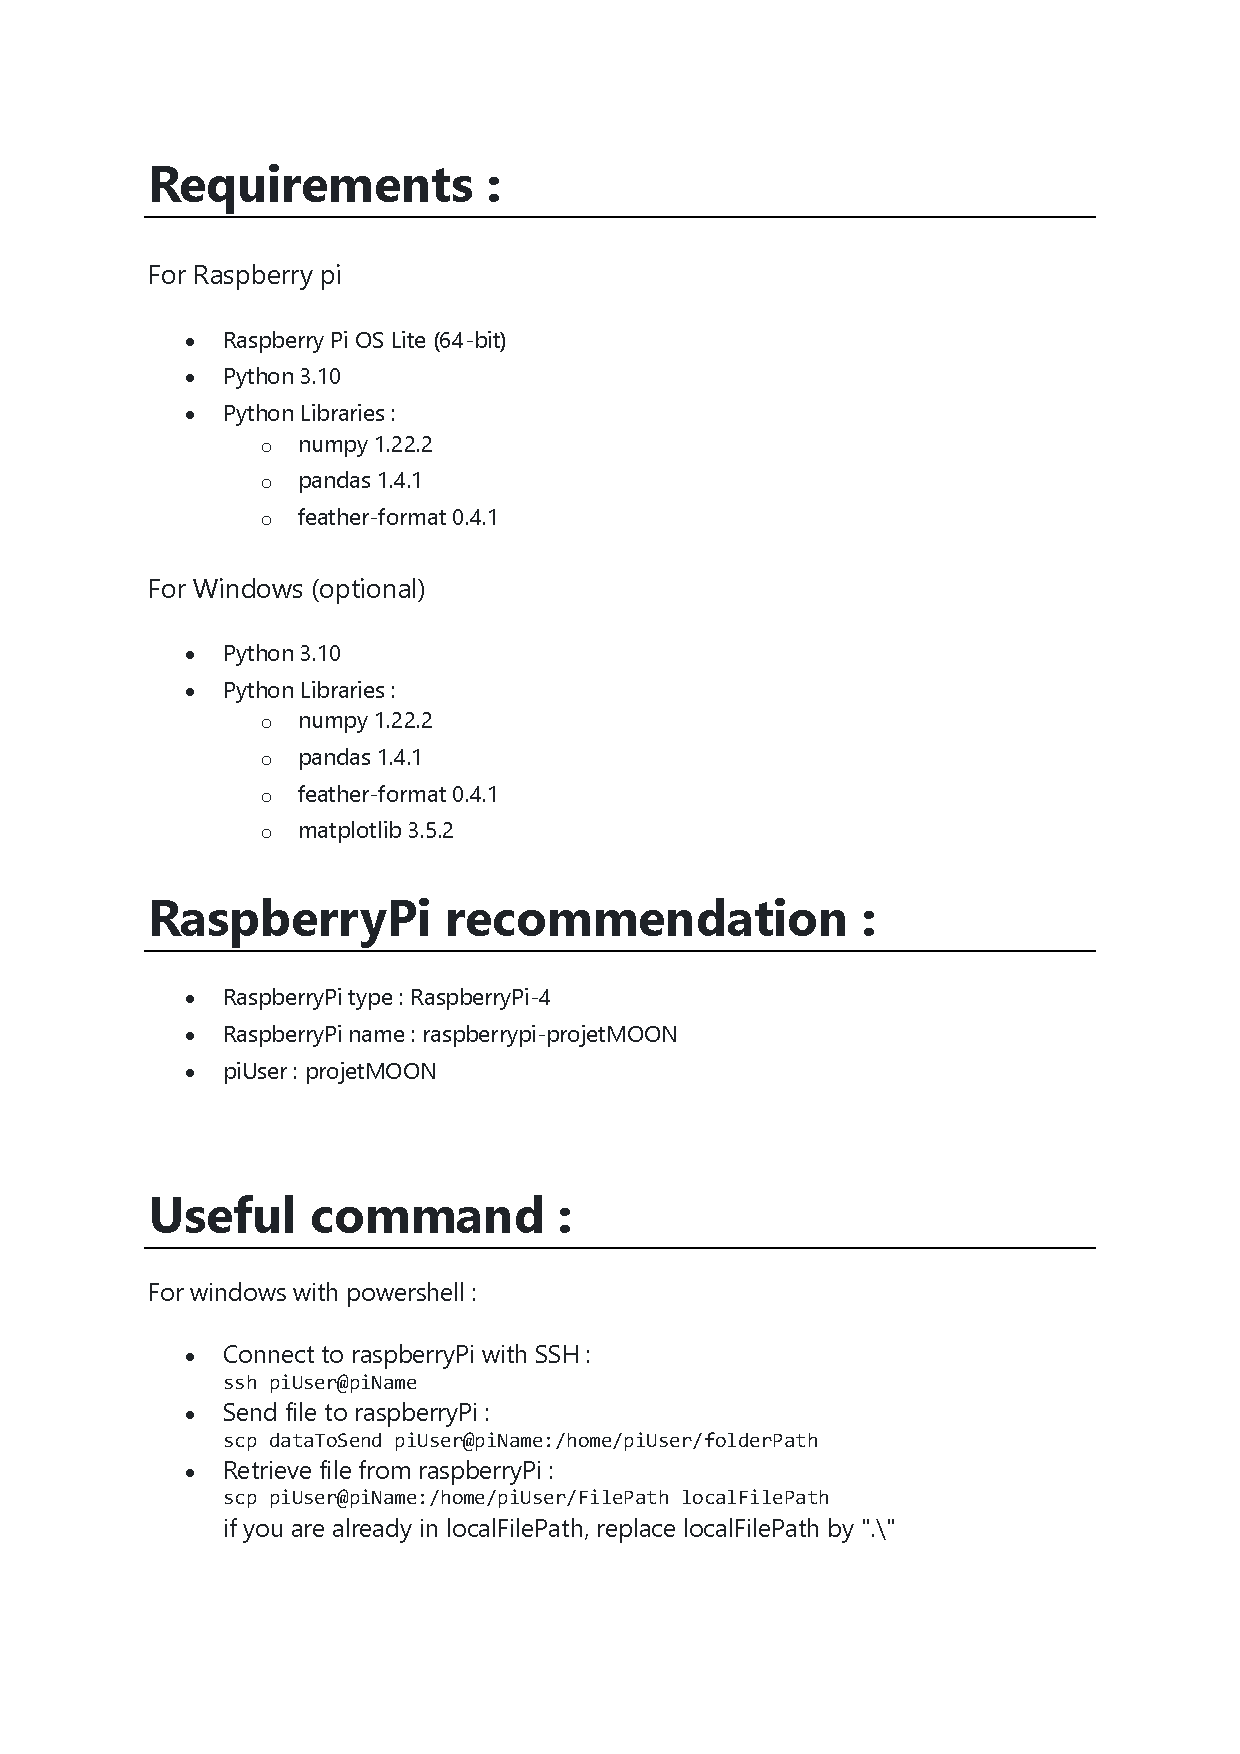
\includepdf[pages={1-11}]{../GuideUtilisateur.pdf}
%
%\newpage
\printbibliography

\end{document}